%!TEX root = pset2.tex

\section{Logistic Regression}\label{sec:lr}

\subsection{Implementation}
We implemented $L_2$-regularized logistic regression using gradient descent.

\subsection{Testing in data with $\lambda = 0$}
We test the logistic regression 

\begin{figure}[h!]
\centering
    \begin{subfigure}[b]{0.4\textwidth}
	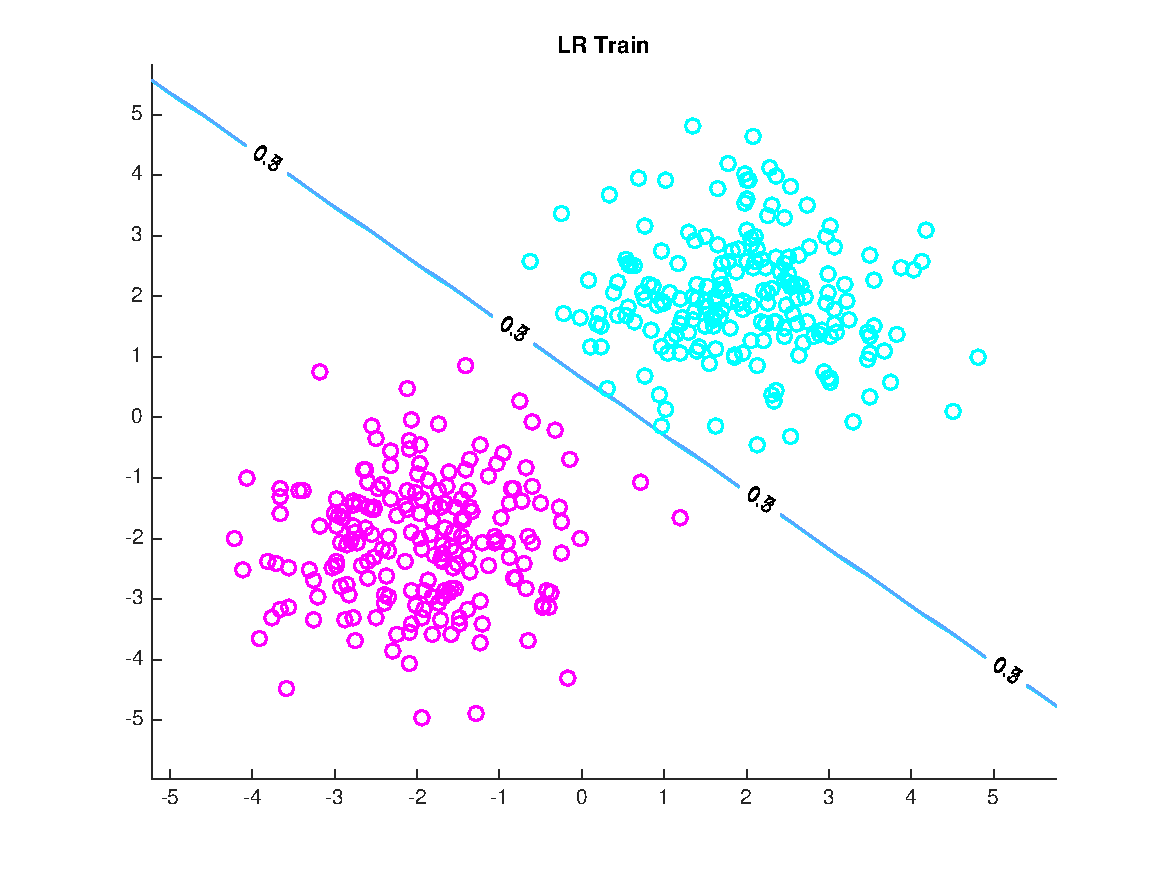
\includegraphics[scale=0.4]{hw2_1_stdev1_a.pdf}
	\caption{Data with $\sigma = 1$, training}\label{fig:data_stdev1a}
    \end{subfigure}
    \quad
    \begin{subfigure}[b]{0.4\textwidth}
	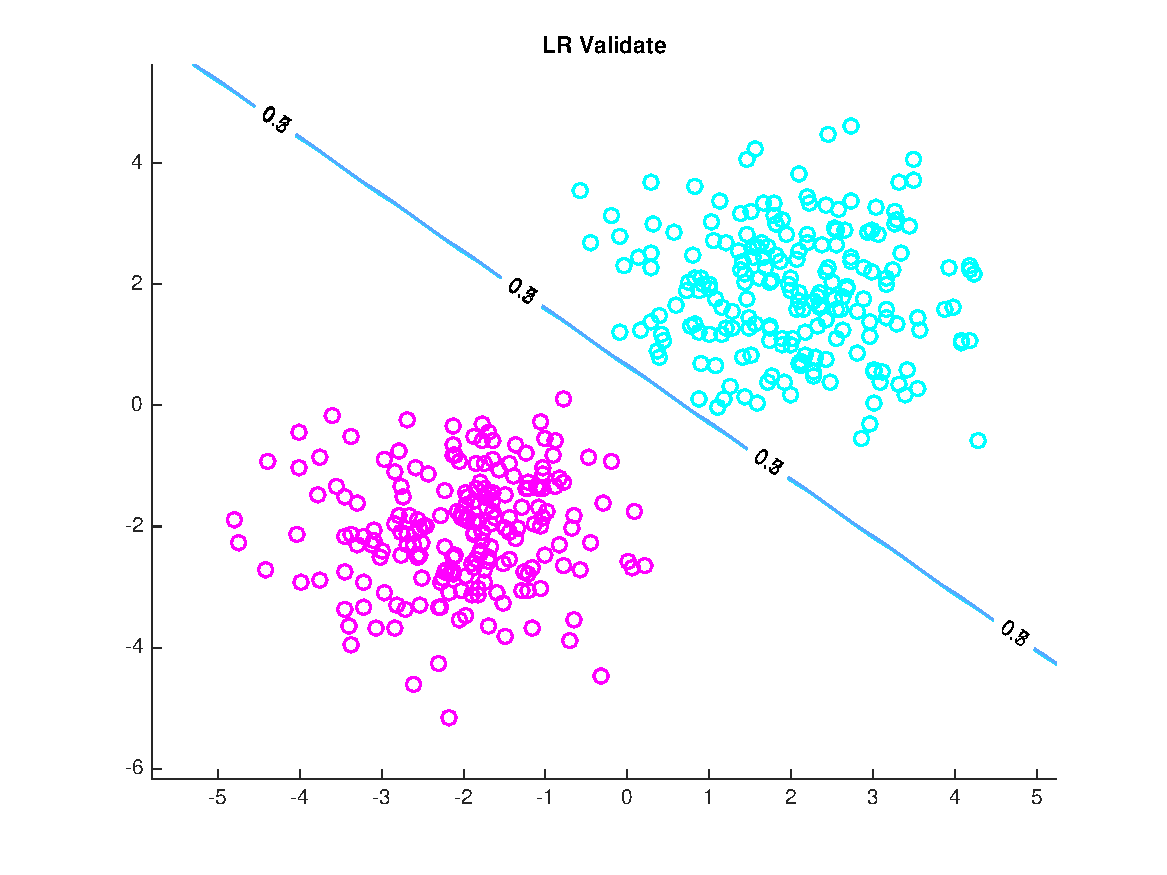
\includegraphics[scale=0.4]{hw2_1_stdev1_b.pdf}
	\caption{Data with $\sigma = 1$, validation}\label{fig:data_stdev1b}
    \end{subfigure}

    \begin{subfigure}[b]{0.4\textwidth}
	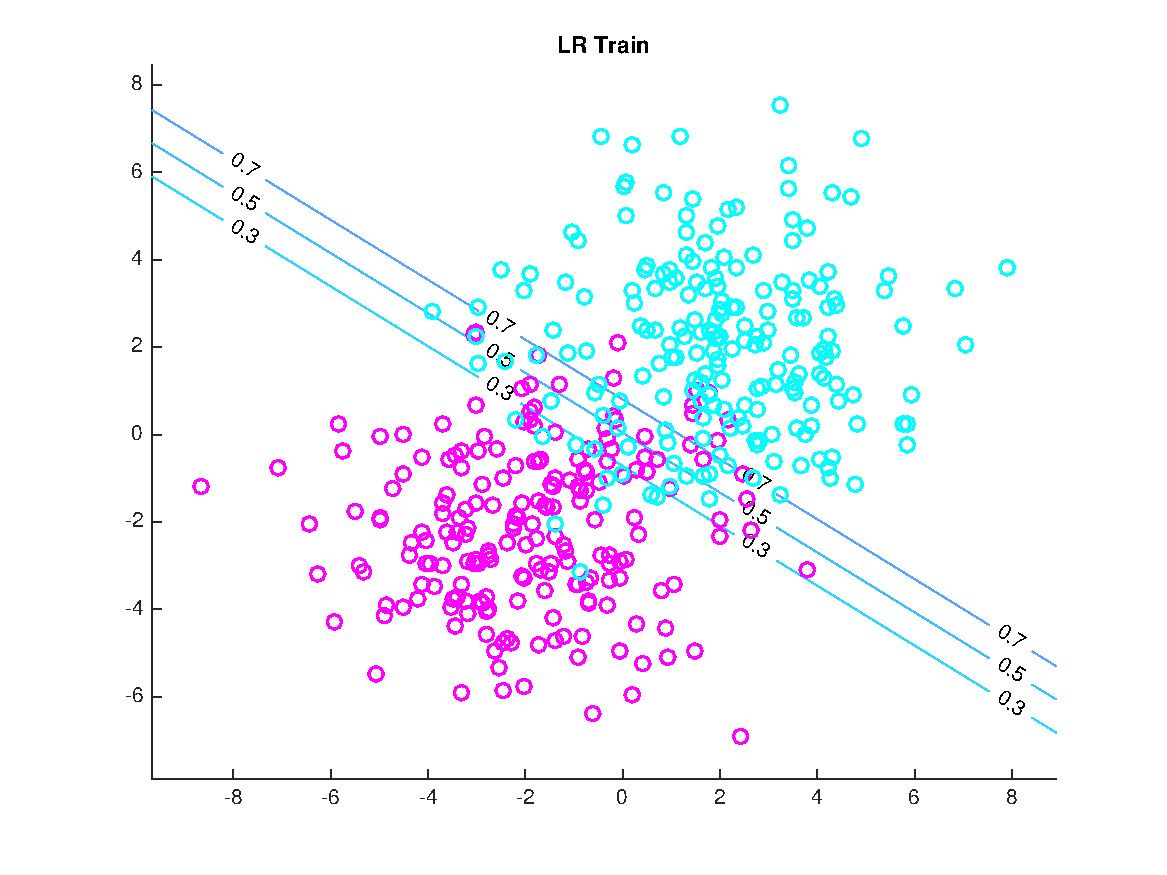
\includegraphics[scale=0.4]{hw2_1_stdev2_a.pdf}
	\caption{CData with $\sigma = 2$, training}\label{fig:data_stdev2a}
	\end{subfigure}
	\quad	
	\begin{subfigure}[b]{0.4\textwidth}
	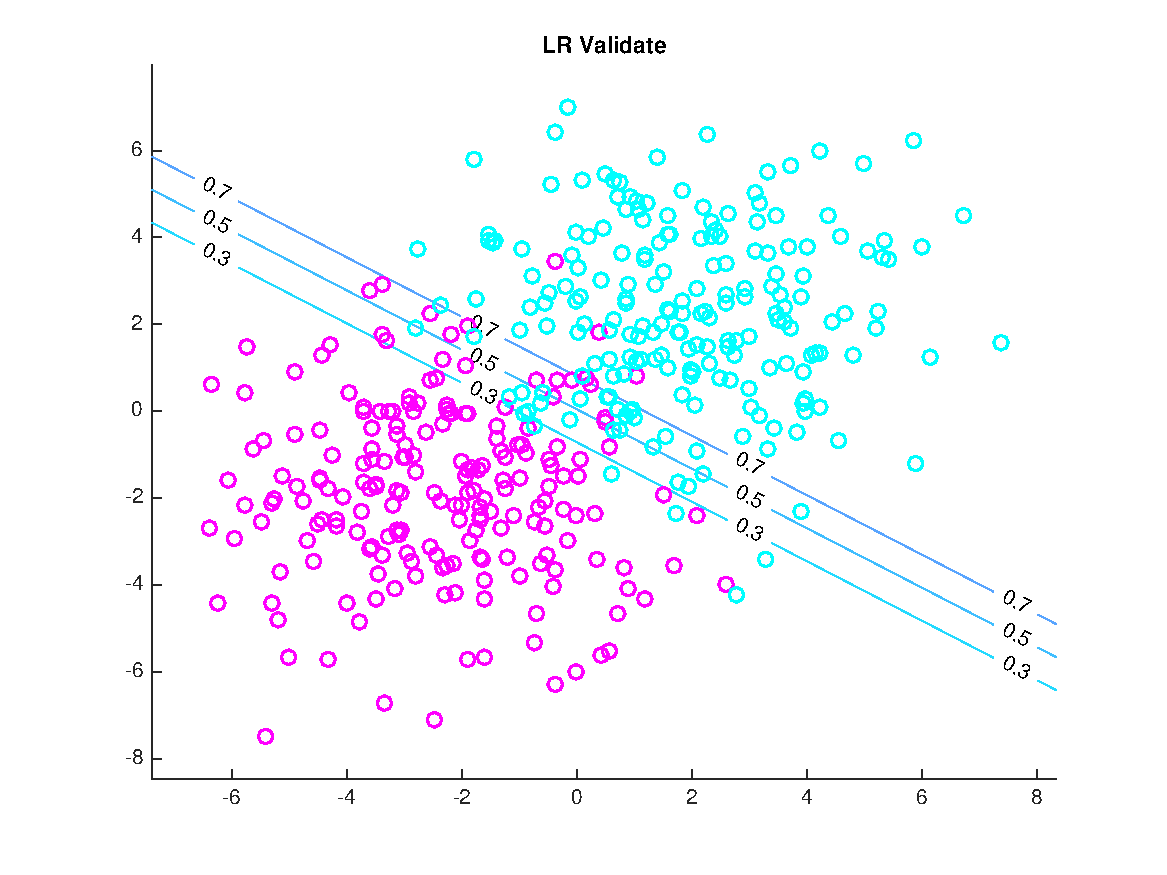
\includegraphics[scale=0.4]{hw2_1_stdev2_b.pdf}
	\caption{CData with $\sigma = 2$, validation}\label{fig:data_stdev2b}
	\end{subfigure}
    
    \begin{subfigure}[b]{0.4\textwidth}
	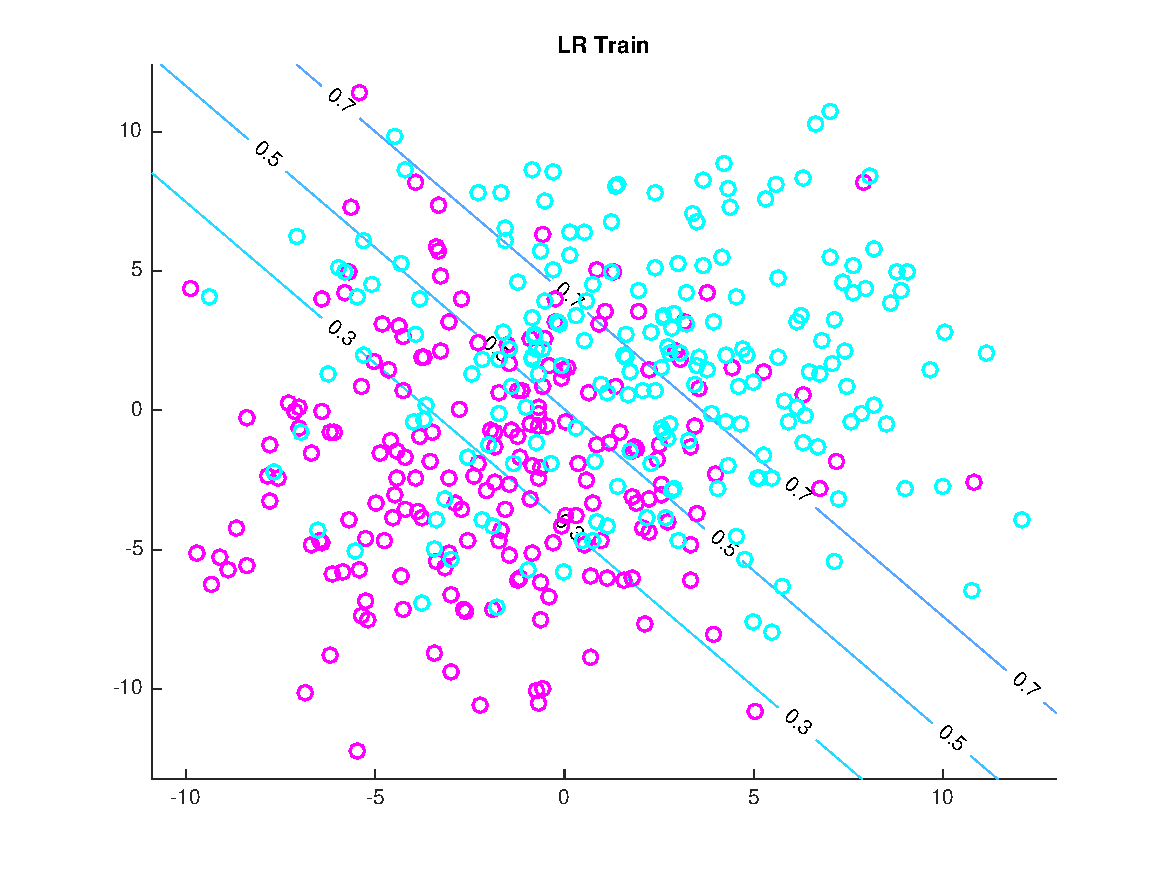
\includegraphics[scale=0.4]{hw2_1_stdev4_a.pdf}
	\caption{Data with $\sigma = 4$, training}\label{fig:data_stdev4a}
    \end{subfigure}  
    \quad
    \begin{subfigure}[b]{0.4\textwidth}
	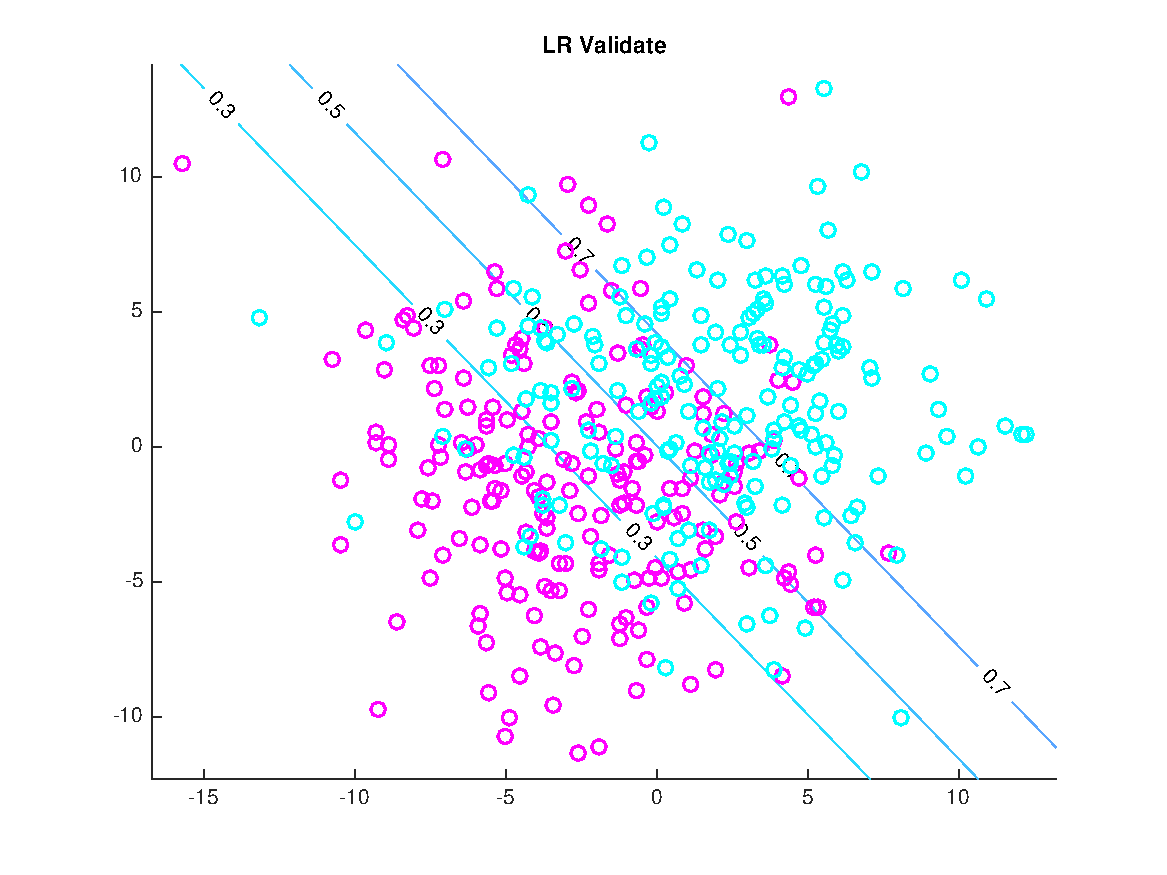
\includegraphics[scale=0.4]{hw2_1_stdev4_b.pdf}
	\caption{Data with $\sigma = 4$, validation}\label{fig:data_stdev4a}
    \end{subfigure}  

    \begin{subfigure}[b]{0.4\textwidth}
	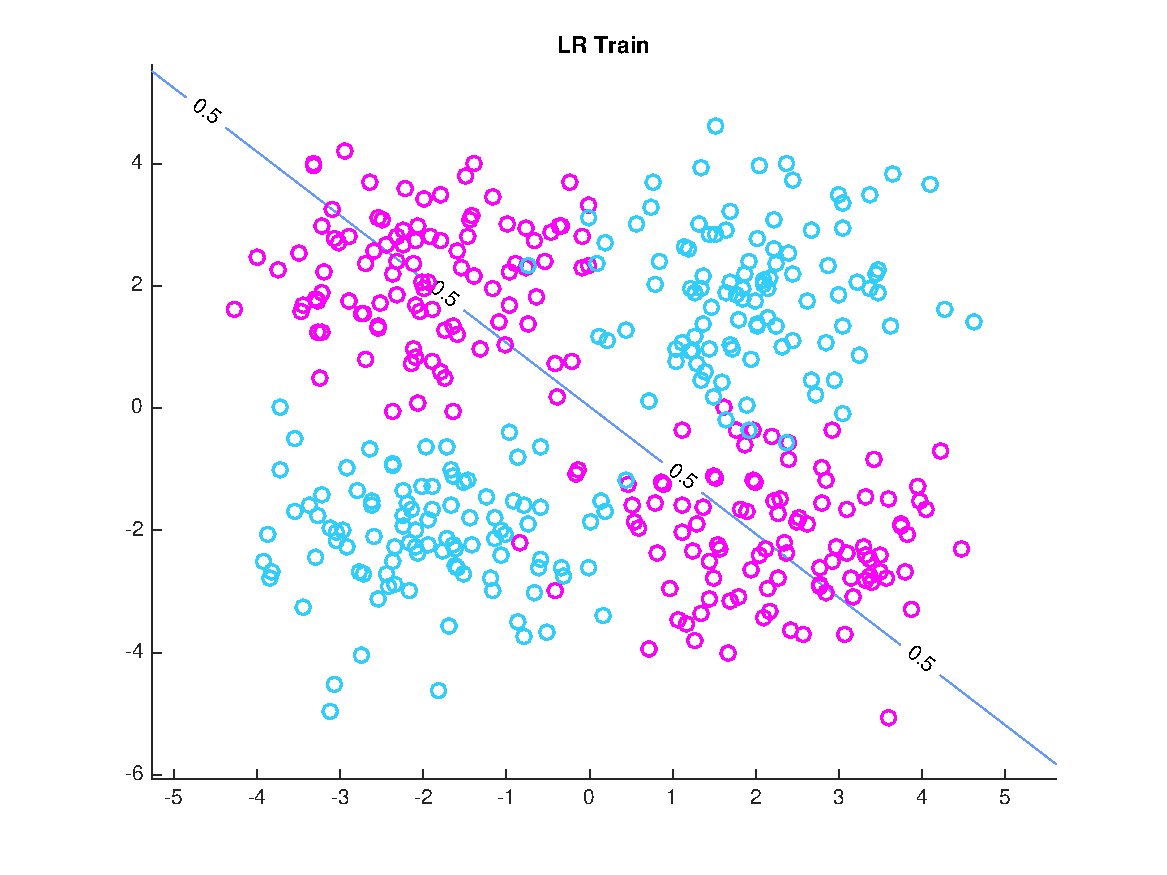
\includegraphics[scale=0.4]{hw2_1_nonsep_a.pdf}
	\caption{Non-seperable data, training}\label{fig:data_nonsep_a}
    \end{subfigure}  
    \quad
    \begin{subfigure}[b]{0.4\textwidth}
	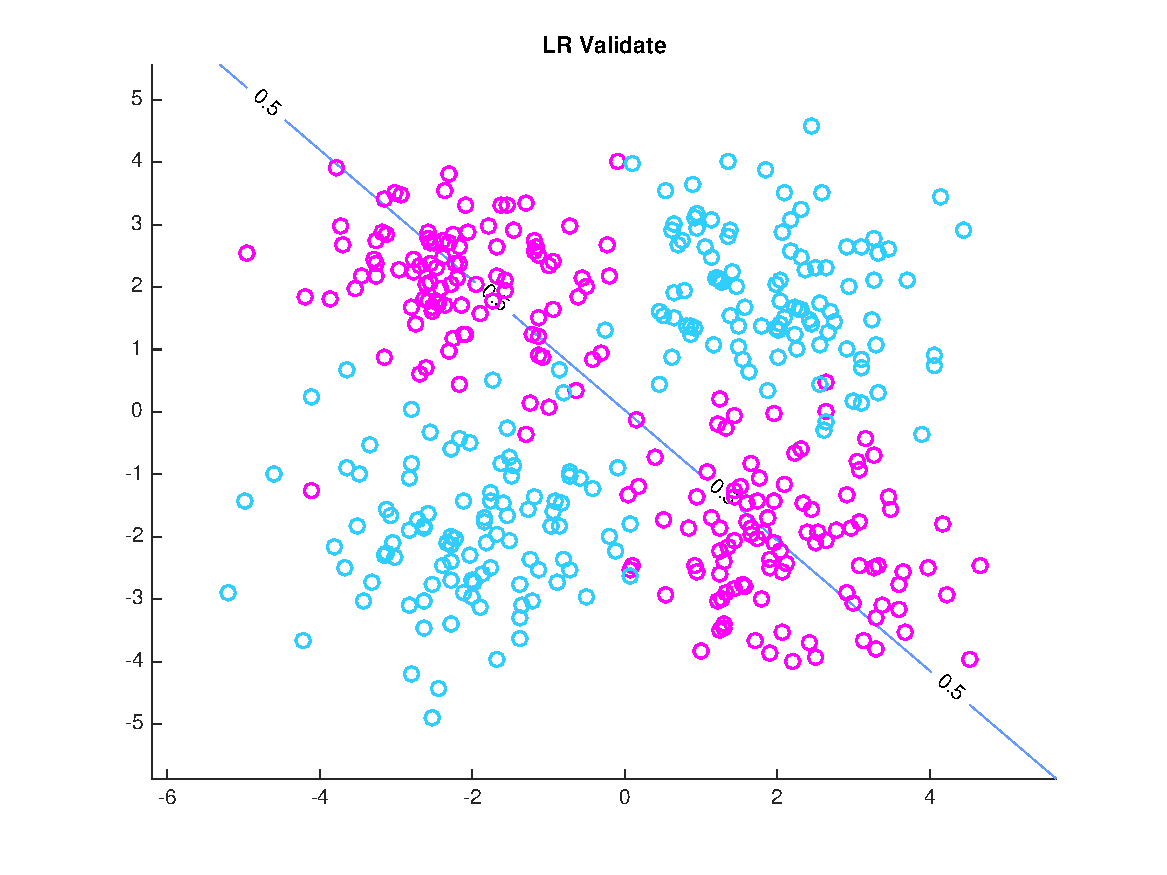
\includegraphics[scale=0.4]{hw2_1_nonsep_b.pdf}
	\caption{Non-seperable data, validation}\label{fig:data_nonsep_b}
    \end{subfigure}  
    \caption{}    
\end{figure}

